\documentclass[fleqn,10pt]{wlscirep}
\usepackage[utf8]{inputenc}
\usepackage[T1]{fontenc}
\usepackage{subcaption}
\usepackage{tikz}
\usepackage{geometry}
\usepackage{nicefrac}
\usepackage{multirow}
\usepackage{gensymb}
\usepackage{multicol}
\usepackage{graphicx}
\usepackage{titlepic}
%\usepackage[demo]{graphicx}
\usepackage{floatrow}
\usepackage{epstopdf}
\usepackage{multirow, booktabs}
%\usepackage[table]{xcolor}

\epstopdfDeclareGraphicsRule{.tga}{png}{.png}{%
  convert #1 \OutputFile
}
\AppendGraphicsExtensions{.tga}

 \geometry{
 left=15mm,
 rmargin = 2 cm
 }
 
%  add marginal notes
\usepackage{marginnote}
\renewcommand\marginfont{%
    \normalfont\scriptsize\itshape
}

% to wrap figures and text
\usepackage{graphicx}
\usepackage{wrapfig}

\usepackage{xcolor}
\definecolor{bgcode}{RGB}{230, 230, 230}  % Bkg color for code block 70 70 70
\usepackage{minted}
\usemintedstyle{sas}  % Style for code block
\usepackage{lmodern}  % To allow bold font inside a code block
\setminted{bgcolor=bgcode} 
%\setminted{bgcolor=bgcode, formatcom=\color{white}} 
\usepackage{fancyhdr}
\pagestyle{fancy}
\fancyhf{} % clear all header and footer fields
\renewcommand{\headrulewidth}{1pt} % Line under header

% \usepackage{nameref}
% \makeatletter
% \newcommand*{\currentname}{\@currentlabelname}
% \makeatother

% \fancyhead[R]{\nouppercas Section \thesection\ \rightmark}} % Section number and name on the right




\DeclareUnicodeCharacter{2212}{-}

\title{Analysis of the H164N mutant $\text{M}^{\text{pro}}$ protein in interaction with the GCP-376 ligand}
\date{}

\author[]{Maurizio Gilioli}

% -----------------------------------------------------------------
% \titlepic{\includegraphics[width=\textwidth]{Images/sfondo.dat.tga}}

\begin{document}

\maketitle
% \begin{tikzpicture}[remember picture,overlay]
%     \node[anchor=north west,yshift=-1.5pt,xshift=1pt]%
%         at (current page. northwest)
%         {\includegraphics[height=15mm]{Images/logoUnitn}};
% \end{tikzpicture}

\tableofcontents

\graphicspath{{images/}}
\newpage
\section{ABSTRACT}


\newpage

\graphicspath{{images/}}

\section{INTRODUCTION}
% !TeX root = ../main.tex
\subsection{Chromatin as the information center of a cell}
All the living organisms possess DNA, which is the main molecule through which information are passed from a generation to another. Chromatin is contained inside the nucleus in an ordered manner
\cite{paroBiologyChromatin2021}
. DNA is wrapped around histones forming nucleosomes. Throughout the report, I will call the nucleomes beads, which is a term that underlines the spherical shape of the DNA-histone complex.
DNA and histones are subjected to different modifications; among those, methylation is the most important modification involving DNA. Methylation in mammals occurs in specific
sites of the genome, called CpGs, where a cyto-
sine is connected directly to a guanine. Methy-
lations of regulatory elements have been im-
plicated in determining cell identity and chro-
matin structure
\cite{liauAdaptiveChromatinRemodeling2017a, shareefExtendedrepresentationBisulfiteSequencing2021}
. CTCF is a protein conserved in eukariotes and is ubiquitous in mammalians
\cite{kimCTCFMultifunctionalProtein2015a}
. It contains a Zync-finger which binds to DNA. The act of binding is performed in cooperation with cohesins, and causes the folding of the chromatin.



\subsection{ATAC-sequencing and CTCF sequencing}
ATAC-sequencing is a technology that allows for the identification of open-
chromatin regions 
\cite{buenrostroTranspositionNativeChromatin2013a, grandiChromatinAccessibilityProfiling2022}. In order to work, it requires the addition of TN-5,
a hyper-active transposase. The latter is preloaded with sequencing adapters
\cite{grandiChromatinAccessibilityProfiling2022}
to induce a contempourary reaction of fragmentation and ligation of the pieces released, in
a process called segmentation. The obtained adapted fragments are then amplified and sequenced. Once the reads are generated, a peak-calling algorithm (in our case MACS-2 
\cite{zhangModelbasedAnalysisChIPSeq2008a}
) is used to determine which portions of the genome present ATAC peaks, and areas where there are
significant enrichments of aligned reads with respect to the background. A significant enrich-
ment of reads is possible only in accessible regions, which are generally also the most active
ones and with available sites for transcription factors binding.
CTCF data, named in chapter ..., were obtained through a classical CHIP-sequencing.
% !TeX root = ../main.tex

\subsection{Chromatin Coarse-Graining, chromatin as a polymeric fluid}

The Young's modulus ($E$) of a chain is the extent to which a solid material (or a polymeric fluid, in this case) can be deformed
As Robert Hook noticed, the following is valid 
\begin{equation}
    \sigma = E \frac{\Delta l}{l}
\end{equation}
Where $l$ represents the length of the chain and $\Delta l$ the deformation $\sigma$
\cite{grosbergGiantMoleculesHere2011}

The entanglement length ($N_e$) corresponds to the Young's modulus that is experimentally found in the plateau region where a force starts to produce irreversible deformations in a chain.

% #TODO put a reference image if you want


It is also defined as the "the average number of monomer units along the chain between two nearest effective cross-links."
and is related to the ability of chains to form knots between each other
\cite{grosbergGiantMoleculesHere2011}
.

%#TODO add subchapter rosettes


\subsubsection{Persistence length of a polymer chain}
%#TODO add subchapter persistence length

The persistence length (\textit{PL}) of a polymer represents the degree of bendability of the chain. During this project, the persistence length is shown in equation \ref{eq: persistence length}.


\begin{equation}
    PL = lk_{CG} / b_{CG} / 2
\end{equation}

With the idea of following a "journey" on the polymer chain, the average angle that you obtain at a contour length $s$ is as in equation \ref{eq: contour length mean angle}. In general, the lower is the contour length analyzed with respect to the persistance length, the higher is the probability of having a low degree angle ($\cos{\theta} \sim 1$). On the contrary, by analyzing larger lengths, it is possible to obtain a wider range of angles.
The concept of persistance length is used in the polymer model to compute the angle bending potentials, which is calculated as in equation \ref{eq: angle bending potential}.


\begin{equation} \label{eq: contour length mean angle}
    \langle \cos{\theta(s)}\rangle = \exp{\left(-\frac{s}{l}\right)}
\end{equation}

\begin{figure}[H] 
    \centering 
    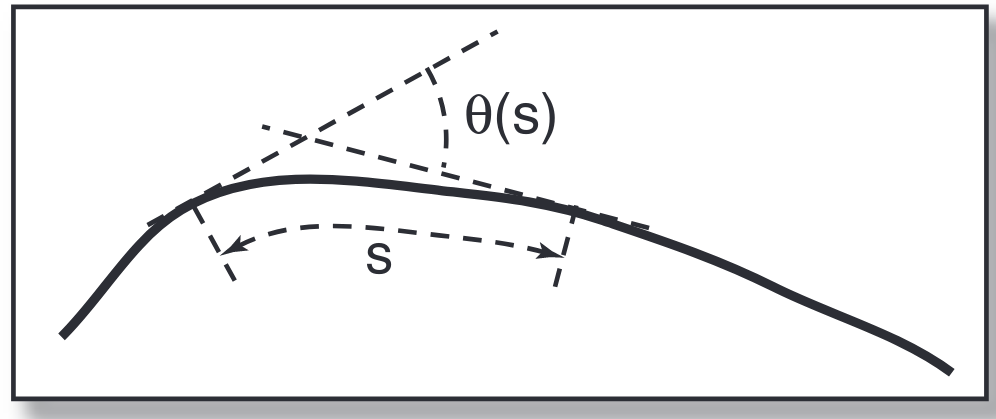
\includegraphics[width=75mm]{persistance_length.png} 
    \caption{Image taken from Grosberg \textit{et al.} 2011\cite{grosbergGiantMoleculesHere2011}. Angle formed between the extremes of a contour length.} 
    \label{examplelabel} 
\end{figure}

%#TODO about the reason of coarse graining with such a low resolution
%#TODO fine scale e coarse grained model, explain reasons

\subsection{\textit{ChromHMM} allows the sequential characterization of chromatin states} \label{intro: chromhmm}
\textit{ChromHMM}
\cite{chilledhousevibesLearningChromatinStates2015}
is a tool which helps in the annotation of genomic DNA by using epigenomic information
\cite{ernstChromatinstateDiscoveryGenome2017}.
It learns chromatin states signatures by using a multivariate hidden Markov model: in each genomic position (segment), it returns the most probable chromatin state and gives other useful information
\cite{chilledhousevibesLearningChromatinStates2015,ernstChromatinstateDiscoveryGenome2017}. 

The package works through two functions in particular, which are the following
\cite{ernstChromatinstateDiscoveryGenome2017}:
\begin{enumerate}
    \item \textbf{\textit{BinarizeBam}}: it converts a set of \textit{.bam} files of aligned reads into binarized data files in a specified output directory. The produced data can be used as input for the \textit{LearnModel} function. When using this command, it has to be specified the segment size, which is set by default to be equal to 200 bps.
    \item  \textbf{\textit{LearnModel}}: it takes a set of binarized data files, learns chromatin state models, and by default produces data reporting the emission/transition parameters of the states, the abundance of the states at the TSSs (Transcriptional Starting Sites), at the TESs (Transcriptional Ending sites), and other relevant portions of the genome (CPG islands, exons, genes). Additionally, a webpage is generated with links to all the files and images created.
\end{enumerate}

\noindent The results obtained from \textit{ChromHMM} are shown in chapter \ref{chap: ChromHMM results}.


% \input{} %#TODO Kremer Grest model explanation
% \input{chapters/intro-hip_hop}

\newpage
\section{Aim of the project} \label{chap: aim}

The project is part of the thesis whose aim is to predict matrices of contact of chromatin through the results obtained with molecular coarse-grained simulations of 2 Mb portions of the chromatin.
The scope of the report is also to gather opinions and useful feedback to improve the thesis work, which will continue for another two months.


\newpage
\section{METHODS}
All the simulations  were performed making use of the simulation software LAMMPS
\cite{LAMMPSDocumentation,steveplimptonLAMMPS},
and some already made codes of Marco di Stefano, researcher at IGH-CNRS (France)

\subsection{Data used during the project} \label{methods: data used}
The data of CTCF and ATAC for the IMR90 cell line, included in the paper written by Jimin and colleagues in 2023
\cite{tanCelltypespecificPrediction3D2023},
were used for the project (see table \ref{tab:data}). It was decided to exploit the same data of \textit{cOrigami} to allow a better comparison between its predictions and those produced by our modelling, which will be done as a last step. Both the two technical replicates, included in the listed ENCODE
\cite{encodeprojectconsortiumIntegratedEncyclopediaDNA2012} 
entries, were considered.

\begin{table}[H]
    \centering
    \begin{tabular}{|c|c|c|}
        \hline
        \textbf{Cell-Type} & \textbf{CTCF ChiP-seq} & \textbf{ATAC-seq}\\
        \hline
        IMR90 & ENCSR000EFI & ENCSR200OML\\
        \hline
    \end{tabular}
    \caption{Table referring to the data used for the analysis.}
    \label{tab:data}
\end{table}

The ATAC-sequencing data were produced following the standard ENCODE procedure
\cite{ATACseqUnreplicatedENCODE}. 
In particular, the processes of read trimming, alignment, and filtering were performed making use of the \textit{Bowtie 2}, \textit{Samtools}, \textit{Sambamba}, \textit{Picard} and \textit{cutadapt} softwares
\cite{michaelcherryATACSeqPipeline}. 
An explanation of the named processes could be found in the work made by Feng Y. and colleagues in 2020
\cite{yanReadsInsightHitchhiker2020}.

When it comes to the ChIP-sequencing data, again, the standard procedure of ENCODE was used to produce the online available datasets. An overview about the method can be found at the following \href{https://www.encodeproject.org/chip-seq/transcription_factor/}{link}
\cite{TranscriptionFactorChIPseq}.
To sum up, at first the reference genome was indexed with the \textit{BWA}, then, the alignments between the reads and the reference genome (\textit{hg38}
\cite{HomoSapiensGenome})
were produced and filtered with the \textit{BWA}, \textit{Samtools}, \textit{Picard}, \textit{BEDTools}, \textit{Phantompeakqualtools} and \textit{SPP} softwares.

%#TODO make a better description of the methods maybe

In the case of our study, the analyzed region included ANPEP, and it was taken from the $89,000,000^{\text{th}}$ base to the $91,000,000^{\text{th}}$ position of the $15^{\text{th}}$ chromosome.


\subsection{Finding enriched states in 5 kbs long beads} \label{methods: finding enriched states}

To find the enriched states in 5 kb long bins, the procedure described in process \ref{algo: enriched states} was followed. The fold change of a state within a bin was determined by dividing the proportion in the bin by the corresponding proportion in chromosome 15. Once done that, the state with the highest fold-change was assigned to the bin. A visual investigation was performed afterwards to check the quality of the "binarization" procedure by using the IGV visualization software
\cite{robinsonIgvJsEmbeddable2020}.

\begin{algorithm}
    \caption{Finding enriched states in 5-kb long bins}\label{algo: enriched states}
    \KwResult{Enriched states}
    \ForAll{chromosomes}{Find proportions of the states in the chromosome}
    \ForEach{bin}{
        Calculate bin proportions for each state\\
        Compute the fold changes\\
        Assign the state with the highest fold change
    }
    Generate .bed files\\
    Visualization in IGV of regions of interests\\
    \tcc{each bin is 5 kb long}
\end{algorithm}

%#TODO maybe it would be the case to talk about other possibilities

% !TeX root = ../main.tex

\subsection{The Model} \label{chap: the model description}
The objective was to create a polymer model with a coarse-graining resolution of 5000 bp.
The model creation was done by using code written by Marco Di Stefano.
The total Genome length was obtained from the UCSC genome browser
\cite{UCSCGenomeBrowser}
. All the simulations were performed making use of periodic boundaries (chapter % \ref{})

All the simulations were performed making use of the \textit{run\_lammps} function inserted in the TADPHYS package. The \textit{bond\_style} that was set for LAMMPS
\cite{thompsonLAMMPSFlexibleSimulation2022}
was the the \textit{fene} bond style whose potential is written in equation \ref{eq: FENE potential}. 

Three types of potential energies were used to regulate the interactions between beads, those potentials are listed below:

\begin{itemize}
    \item \textbf{FENE potential: }The FENE potential is a finite extensible nonlinear elastic potential and is generally used for polymer models. The first term is attractive, the second term is a Lennard-Jones (LJ) potential, and it's repulsive. The first term extends to $R_0$, the maximum extent of the bond. The second term has a cutoff set at $2^{\nicefrac{1}{6}} \sigma$, the minimum of the LJ potential.
    \cite{thompsonLAMMPSFlexibleSimulation2022}
    . The K is an $\frac{\text{energy}}{\text{distance}^2}$ measure

    \begin{equation} \label{eq: FENE potential}
        E = -0.5 K R_0^2 \ln{\left[1 - \left(\frac{r}{R_0}\right)^2\right]} + 4 \epsilon \left[\left(\frac{\sigma}{r}\right)^{12} - \left(\frac{\sigma}{r}\right)^6\right] + \epsilon
    \end{equation}

    The following specifications were made for the FENE interactions:

    \begin{enumerate} %#TODO unit of measures
        \item 30.0: Maximum force the bond can withstand. It represents the stiffness or strength of the bond.
        \item 1.5: Maximum extension of the bond. This is the maximum distance at which the bond can be stretched.
        \item 1.0: Equilibrium bond length. This is the ideal or equilibrium distance between the bonded particles.
        \item 1.0: Bond force constant. It affects how quickly the potential energy increases as the bond length deviates from the equilibrium length.
    \end{enumerate}

    \item \textbf{Excluded-volume interactions: } To allow for the excluded-volume interactions, a simple Lennard-Jones potential was included, written as in equation %#TODO extend this part

    \begin{align} \label{eq: lennard jones potential}
        E_{LJ} &= 4 \epsilon \left[\left(\frac{r_0}{r}\right)^{12} - \left(\frac{r_0}{r}\right)^6\right]&& r < r_c \nonumber\\
            &= 4 \epsilon \left[\left(\frac{2^{\nicefrac{1}{6}}\sigma}{r}\right)^{12} - \left(\frac{2^{\nicefrac{1}{6}}\sigma}{r}\right)^6\right]&& r < r_c 
    \end{align}


    Three parameters are set:

    \begin{enumerate} %#TODO units of measure
        \item $\epsilon$ (energy unit): 1.0, Note that $\sigma$ is defined in the LJ formula as the zero-crossing distance for the potential, not as the energy minimum at $r_0 = 2^{\nicefrac{1}{6}} \sigma$ .
        \item $\sigma$ (distance unit): 1.0
        \item LJ cutoff (distance unit): 1.12246152962189
    \end{enumerate}

    \item \textbf{Angle bending potentials: }The angle bending associated potentials are directly correlated with the persistence length (PL), which is calculated as in equation \ref{eq: persistence length}.

    \begin{equation} \label{eq: persistence length}
        PL = lk_{CG} / b_{CG} / 2
    \end{equation}

    The angle potentials are given to LAMMPS and calculated setting the $K$ parameter in equation \ref{eq: angle bending potential}. The larger is the value of K, the larger is in general the potential associated to the angles.

    \begin{equation} \label{eq: angle bending potential}
        E = K[1 + \cos{(\theta)}]    
    \end{equation}

\end{itemize}


The steps performed will be described in the following paragraphs:

%%%%%%%%%%%%%%%%%%%%%%%%%%%%%%%%%%%%%%%%%%%%%%%%%%%%%%%%%%%%%%%%%%%%%%%%%%%%%%%%%%%%%%%%%%%%%%%%%%%
% FOLDER 00a_coarse_graining
%%%%%%%%%%%%%%%%%%%%%%%%%%%%%%%%%%%%%%%%%%%%%%%%%%%%%%%%%%%%%%%%%%%%%%%%%%%%%%%%%%%%%%%%%%%%%%%%%%%

\paragraph{The computation of the parameters for Coarse Graining:}

Both parameters for the fine-scale model (table \ref{tab: parameters FS}) and the CG model (table \ref{tab: parameters CG}) were calculated. The number of bp wrapping around a bead in the FS method was considered to be 150, while instead the linker portion was considered to be of length 50 bp (table \ref{tab: parameters FS}). The thickness of a bead (of a nucleosome) was taken as equal to 10 nm, while instead the default Kuhn length was set to 50 nms. The genome densities ($\rho_{FS} = \rho_{CG} = 0.012\; \text{bp}/\text{nm}^3$) are imposed to be the same for the FS and the CG model.

%#TODO reference!
.
The beads and bonds have all the same length, consequently, the contour length is exactly the product between the number of beads and the size of the beads in the FS and in the CG model. The DNA content was 2000000 bp. To find the parameters for the CG model, the DNA content of the Kuhn segments ($Dlk_{CG}$) were tuned to match the desired value of DNA content in CG beads ($\nu_{CG}$).

%#TODO what is c?

\begin{table}[H]

\begin{tabular}{|l|l|c|}
\hline
\textbf{Property} & \textbf{Formula} & \textbf{Value}\\
\hline
\textbf{$c$} & \textit{const.} & 19\\
\hline
\textbf{$\nu_{FS}$} (DNA content of a monomer in b.) & \textit{const.} & 150+50 bp = 200 bp\\
\hline
\textbf{$b_{FS}$} (Diameter of a bead in nm) & \textit{const.} & 10 nm\\
\hline
\textbf{$lk_{FS}$} (Kuhn length of the chain  in FS) & \textit{const.} & 50 nm \\
\hline
\textbf{$\rho_{FS}$} (Genome density) &\textit{const.} & $0.012\; \text{bp}/\text{nm}^3$ \\ %#TODO da dove?
\hline
\textbf{$N_{FS}$} (Number of monomers to represent the chromosome) & $\frac{\text{DNAcontent}}{\nu_{FS}} * \text{ncopies}$ & 30000 mon.\\
\hline
\textbf{$N^k_{FS}$} (Number of Kuhn lengths of the chain) & $\frac{N_{FS} * b_{FS}}{lk_{FS}}$ & 6000 k. l.\\
\hline
\textbf{$\rho^k_{FS}$} (Genome density in Kuhn lengths) & $\frac{\rho_{FS} \cdot b_{FS}}{\nu_{FS} \cdot \text{lk}_{FS}}$& $1.2e-05$ 1/nm³\\
\hline
\textbf{$L_{FS}$} (Polymer contour length) & $N_{FS} * b_{FS}$ & 300000 nm\\
\hline
\textbf{$Le_{FS}$} (Entanglement length of the chain in nm) & $lk_{FS} * \left(\frac{c}{\rho^k_{FS} * lk_{FS}^3}\right)^2$ & 8022.22 nm\\
\hline
Number of monomers in a Kuhn length FS & $lk_{FS}/b_{FS}$ & 5 mon.\\
\hline
$Blk_{FS}$ (Bead content of a Kuhn length FS) & $(lk_{FS} \cdot b_{FS})/\nu_{FS}$ & 2.5 $\text{nm}^2$/bp  \\
\hline
$Dlk_{FS}$ (DNA content of a Kuhn length FS) & $(lk_{FS} \cdot \nu_{FS})/b_{FS}$ & 1000 $\text{bp}$\\
\hline
\end{tabular}
\label{tab: parameters FS}
\caption{Parameters calculated for the Fine Scale (FS) model}
\end{table}

%%%%%%%%%%%%%%%%%%%%%%%%%%%%%%%%%%%%%%%%%%%%%%%%%%%%%%%%%%%%%%%%%%%%%%%

\begin{table}[H]
    \begin{tabular}{|l|c|c|}
        \hline
        \textbf{Property} & \textbf{Formula} & \textbf{Value}\\
\hline
\textbf{$c$} & \textit{const.} & 19\\
\hline
$\nu_{CG}$ (DNA content of a monomer in b.) & \textit{const.} & 5000 bp\\
\hline
$Dlk_{CG}$ (DNA content of a Kuhn length CG) & \textit{tuned const.} & 33791 bp\\
\hline
$\phi_{CG}$ (Volumetric density of the chain in the CG model for IMR90 cell-type) & \textit{const.} & $0.1$ \\ %#TODO che MEASURE ha?
\hline
\textbf{$\rho_{CG}$} (Genome density in bp/nm³) & \textit{const.} & $0.012\; \text{bp}/\text{nm}^3$\\
\hline
$b_{CG}$ (Diameter of a bead in nm) & $\sqrt{\left(\sqrt{\frac{{Dlk_{CG}}}{{Blk_{FS}}}}\right) / \rho_{CG} \cdot \frac{6}{\pi} \cdot \phi_{CG}}
$ & 43.0155 nm\\
\hline
\textbf{$lk_{CG}$} (Kuhn length of the chain  in CG) & $\sqrt{Dlk_{CG} * Blk_{FS}}$ & 290.65 nm \\
\hline
Number of monomers in a Kuhn length CG & $lk_{CG}/b_{CG}$ & 6.75687 mon.\\
\hline
\textbf{$N_{CG}$} (Number of monomers to represent the chromosome) & $\frac{\text{DNAcontent}}{\nu_{CG}} * \text{ncopies}$& 1200 mon.\\
\hline
$\text{side}_{CG}$ (size of the cubic simulation box) & $\frac{{(N_{CG} \cdot \nu_{CG} / \rho_{CG})^{1/3}}}{{b_{CG}}}
$ & 18.4515 nm\\
\hline
\textbf{$N^k_{CG}$} (Number of Kuhn lengths of the chain) & $(N_{CG} * b_{CG})/{lk_{CG}}$ & 177.597 k. l.\\
\hline
\textbf{$\rho^k_{CG}$} (Genome density in Kuhn lengths bp/nm) & $\frac{\rho_{CG} \cdot b_{CG}}{\nu_{CG} \cdot \text{lk}_{CG}}$ & $3.55194$e-07 \nicefrac{bp}{nm} \\
\hline

\textbf{$L_{CG}$} (Polymer contour length) & $N_{CG} * b_{CG}$& 51618 nm\\
\hline
\textbf{$Le_{CG}$} (Entanglement length of the chain in nm) & $lk_{CG} * \left(\frac{c}{\rho^k_{CG} * lk_{CG}^3}\right)^2$ & 1379.51 nm\\
\hline
\end{tabular}
\label{tab: parameters CG}
\caption{Parameters calculated for the coarse-grained (CG) model}
\end{table}

%#TODO how do you find the side?
%#TODO inserire chromatin_volumetric_density.sh?


%%%%%%%%%%%%%%%%%%%%%%%%%%%%%%%%%%%%%%%%%%%%%%%%%%%%%%%%%%%%%%%%%%%%%%%%%%%%%%%%%%%%%%%%%%%%%%%%%%%
% CARTELLA 00_generate_initial_conformation_rosette
%%%%%%%%%%%%%%%%%%%%%%%%%%%%%%%%%%%%%%%%%%%%%%%%%%%%%%%%%%%%%%%%%%%%%%%%%%%%%%%%%%%%%%%%%%%%%%%%%%%

\paragraph{Generation of the initial conformation rosettes:}

Once found the coarse graining parameters, rosettes for 100 replicates were built, with a radius of 12.0 nm inside a cubic box of 300 nm. The particle radius was set to 0.5 nm. In each replicate, three equal chains were built, by setting a different random seed each time. The total number of particles in each chain was of 400 beads.


%%%%%%%%%%%%%%%%%%%%%%%%%%%%%%%%%%%%%%%%%%%%%%%%%%%%%%%%%%%%%%%%%%%%%%%%%%%%%%%%%%%%%%%%%%%%%%%%%%%
% CARTELLA 01_compression_to_desired_phi_rosette
%%%%%%%%%%%%%%%%%%%%%%%%%%%%%%%%%%%%%%%%%%%%%%%%%%%%%%%%%%%%%%%%%%%%%%%%%%%%%%%%%%%%%%%%%%%%%%%%%%%

\paragraph{Finding the optimal pressure:}

Once the rosettes were made, a decompaction was performed starting from the compacted rosettes. A range of values of pressure was tested from 0.1 to 1 with steps every 0.1. For each replicate, a new random seed was generated and stored.
Before attempting the decompression, the minimal energy structure was found by taking into consideration a stopping energy tolerance of $1*10^{-4}$, a stopping tolerance force of $1*10^{-6}$, a maximal number of iterations and evaluations of 100000 steps. %#TODO maybe chiarisci questo
The process was long 1000 steps with a duration of \SI{0.001}{\pico\second}. %#TODO is it correct?
and the final structure was taken as the decompressed one.
The optimal pressure was attested at 0.192 %#TODO what measure



%#TODO chiarisci faccenda angle style e angle value
%#TODO put figures about pressure.

% \begin{figure}[H]
%     \centering
%     % \includegraphics{images}
%     \caption{Pressure values associated to the corresponding resulting box sides for the first 10 replicates are depicted. The target value for the side of the box is indicated by the red dashed line and is equal to 18.4515 nm (table \ref{tab: parameters CG}). The corresponding pressure was taken for the next steps. The optimal pressure was attested at 0.192} %#TODO add unit of measure
%     \label{fig:enter-label}
% \end{figure}


%%%%%%%%%%%%%%%%%%%%%%%%%%%%%%%%%%%%%%%%%%%%%%%%%%%%%%%%%%%%%%%%%%%%%%%%%%%%%%%%%%%%%%%%%%%%%%%%%%%
% CARTELLA 02_estimate_time_conversion_rosette
%%%%%%%%%%%%%%%%%%%%%%%%%%%%%%%%%%%%%%%%%%%%%%%%%%%%%%%%%%%%%%%%%%%%%%%%%%%%%%%%%%%%%%%%%%%%%%%%%%%

\paragraph{Decompaction and relaxation:}

Once the optimal value for the pressure was found (0.192) %#TODO unit of measure
for each replicate, other two simulations respectively $5,000,000$ and $25,000,000$ steps long were performed (not after a minimization phase). This time, the step was set to have a temporal length of \SI{0.0012}{\pico\second} In both the cases MSD values were collected every 100 steps. A frame was dumped every 5000 steps. At the end, the trajectories were collected and analyzed by computing the \textit{RMSD}, \textit{Rg} and the autocorrelation function as described in chapter \ref{chap: trajectory analysis}. For the sake of simplicity, the collection was accomplished by capturing one frame for every 50,000 steps.

%%%%%%%%%%%%%%%%%%%%%%%%%%%%%%%%%%%%%%%%%%%%%%%%%%%%%%%%%%%%%%%%%%%%%%%%%%%%%%%%%%%%%%%%%%%%%%%%%%%
% CARTELLA 03_estimate_time_conversion_rosette
%%%%%%%%%%%%%%%%%%%%%%%%%%%%%%%%%%%%%%%%%%%%%%%%%%%%%%%%%%%%%%%%%%%%%%%%%%%%%%%%%%%%%%%%%%%%%%%%%%%

\paragraph{Computing matrices of contact:}

Once defined the step at which the simulations were considered to be at the equilibrium, some dictionaries produced with \textit{ChromHMM}
\cite{chilledhousevibesLearningChromatinStates2015,ernstChromatinstateDiscoveryGenome2017}
, by using CTCF and ATAC-seq data, were used to define the identity of the beads. During the next steps, we will try to select the best attraction parameters; the stepwise algorithm \ref{algo: comparison} is being currently tested. All the beads were considered to have a radius of 0.5 %#TODO unit of measure
long. To quantify attraction potentials, a new Lennard-Jones potential was added (as defined in equation \ref{eq: lennard jones potential}). In particular, the cutoff distance $r_0$ was set to be equal to:

$$
r_0 = r_{\text{cutoff}} = \sigma * 2.5
$$

% repulsion interactions
% $$
% r_0 = r_{\text{cutoff}} = 3 * 2^{\nicefrac{1}{6}}
% $$

Once the interaction parameters are set, other 1 second long simulations are performed with the intention of generating contact maps. Only the interactions occurring intra-chain were considered. 
%#TODO how and when there is a contact?


% #TODO non so se aggiungere questo discorso. come vengono assegnate ai bin le biglie?
% #TODO Since the real map and the CG map had different resolutions (5,000 and 10,000 respectively), the beads from the coarse gra 



% #TODO PUT A COMMENT TO SUMMARIZE EVERYTHING
% \begin{important}
%     ciao
% \end{important}



% !TeX root = ../main.tex
\subsection{Trajectories analysis} \label{chap: trajectory analysis}

Three types of analysis were performed (all the terms are explained in the Glossary): %#TODO don't know if it's necessary to specify this

\begin{enumerate}
    \item \textbf{\textit{RMSD}}: The Root Mean Square Deviation is calculated by using the \textit{MDanalysis} package
    \cite{gowersMDAnalysisPythonPackage2016}
    and is calculated as follows:

    \begin{equation} \label{eq: RMSD}
        RMSD = \rho(t) = \sqrt{\frac{1}{N} \sum_{i=1}^N{w_i \left(\vec{x_i}(t) - \vec{x_i}^{REF}\right)^2}}
    \end{equation}

    Before performing this type of calculation, the structures were aligned to the first frame (each frame of each replicate was aligned to the first frame of their specific replicate). This type of alignment was done making use of the \textit{AlignTraj} function
    \cite{gowersMDAnalysisPythonPackage2016}
    . In general, the smaller is the difference between two structures, the lower is the value of RMSD. The results are written in graph
    
    \begin{figure}
        \centering
        
        \begin{subfigure}{0.49\textwidth}
          \includegraphics[width=\linewidth]{/home/maurizio/Documents/GitHub/3DCS/Maurizio/steps/5-extract_info_trajectories/images/rmsd_1_IMR90.png}
          \caption{Graph representing the RMSD of the chains pertaining to the first replicate. As it is possible to see from the legend, the first, the second and the third chain are represented respectively in blue orange and green.}
          \label{fig:RMSD first replicate}
        \end{subfigure}
        \hfill
        \begin{subfigure}{0.49\textwidth}
          \includegraphics[width=\linewidth]{/home/maurizio/Documents/GitHub/3DCS/Maurizio/steps/5-extract_info_trajectories/images/rmsd_50000_IMR90_modified.png}
          \caption{Figure representing the collective behaviour of all the chains of all the 100 replicates. It is possible to observe a plateau at approximately $50*50000$ steps. The red dashed line represents the average value.}
          \label{fig:RMSD collective replicates}
        \end{subfigure}
      
        \caption{RMSD profiles}
        \label{fig:RMSD figures}
    \end{figure}

    %%%%%%%%%%%%%%%%%%%%%%%%%%%%%%%%%%%%%%%%%%%%%%%%%%%%%%%%%%%%%%%%%%%%%%%%%%%%%%%%%%%%%%

    \item \textbf{$R_g$}: The Radius of Gyration computed by \textit{MDanalysis} was calculated as written in equation \ref{eq: radius of gyration}. This quantity is a measure of how the mass of an object is spread out relative to a particular axis of rotation. In general, it tells "how spherical" is an object
    \cite{gowersMDAnalysisPythonPackage2016,tuckermanStatisticalMechanicsTheory2015}
    .
    

    \begin{equation} \label{eq: radius of gyration}
        R_g = \sqrt{\frac{\sum_i{m_i \vec{r_i}^2}}{\sum_i{m_i}}}    
    \end{equation}
    

    \begin{figure}
        \centering
        
        \begin{subfigure}{0.49\textwidth}
          \includegraphics[width=\linewidth]{/home/maurizio/Documents/GitHub/3DCS/Maurizio/steps/5-extract_info_trajectories/images/radius_gyr_1_IMR90.png}
          \caption{Graph representing the $R_g$ of the chains pertaining to the first replicate. As it is possible to see from the legend, the first, the second and the third chain are represented respectively in blue orange and green.}
          \label{fig:RG first replicate}
        \end{subfigure}
        \hfill
        \begin{subfigure}{0.49\textwidth}
          \includegraphics[width=\linewidth]{/home/maurizio/Documents/GitHub/3DCS/Maurizio/steps/5-extract_info_trajectories/images/radius_gyr_50000_IMR90_modified.png}
          \caption{Figure representing the collective behaviour of all the chains of all the 100 replicates. The red dashed line represents the average value.}
          \label{fig:RG collective replicates}
        \end{subfigure}
      
        \caption{$R_g$ profiles}
        \label{fig:RG figures}
    \end{figure}


    \item \textit{\textbf{Autocorrelation function:}} The autocorrelation function can be written as shown in equation \ref{eq: autocorrelation}
    \cite{sumaElectricFieldDrivenTrappingPolyelectrolytes2018}
    . Results are shown in %#TODO aggiungi immagine
    
    \begin{equation} \label{eq: autocorrelation}
      r_k = \frac{C_k}{C_0} = \frac{\frac{1}{M} \sum_{t = 1}^{M - k}{(A_t - \bar{A})(A_{t+k} - \bar{A})}}{\frac{1}{M} \sum_{t = 1}^{M - k}{(A_t - \bar{A})^2}}
    \end{equation}

    Where $C_k = \frac{1}{M} \sum_{t = 1}^{M - k}{(A_t - \bar{A})(A_{t+k} - \bar{A})}$ is the autocovariance function at lag k and $C_0 = \frac{1}{M} \sum_{t = 1}^{M - k}{(A_t - \bar{A})^2}$ is the variance function.
    

\end{enumerate}

% !TeX root = ../main.tex
\subsection{Algorithms used for comparison}


As stated in the methods section \ref{chap: the model description} about the simulations, the attraction potentials are sequentially added to the model in order to improve the predictions. The SCC metric was used to compute the difference between the control contact matrix and the CG derived one (chapter \ref{chap: SCC method}).

Two methods were then considered to add the variables, which are expressed in algorithm \ref{algo: greedy comparison} and \ref{algo: comparison}. Since the states are differentially populated, as stated in chapter \ref{chap: ChromHMM results}, it is possible to argue that the largest contribution to the result would be given, in a hierarchical manner, by the most populated states. As a consequence of this consideration, I could fix the values related to the most prevalent states, before considering those that are less present. This type of mechanism is described in the greedy process of algorithm \ref{algo: greedy comparison}. If that assumption is not accepted, then either you test all the possible configurations, either you find a better way to test the generated models. The algorithm \ref{algo: comparison} is a stepwise solution which allows to solve partially the problem at the cost of more simulations to perform. \\

\begin{algorithm}[H]
    \caption{Greedy matrix comparison}\label{algo: greedy comparison}
    \KwResult{Best performing greedy model}
    \ForAll{attraction parameter}{
        Construct models by adding the most present attraction parameter to the $(n-1)^{\text{th}}$ step configuration \;
        Compute SCC of the model with respect to the reference ranging among a list of possible values\;
        Select the value of the parameter which gives the best results\;
        Add that attraction with that coefficient\;
    }
    \Return{Best greedy model}\;
    % \tcc{The states are taken from the most populated to the least populated}
\end{algorithm}

%%%%%%%%%%%%%%%%%%%%%%%%%%%%%%%%%%%%%%%%%%%%%%%%%%%%%%%%%%%%%%%%%%%%%%%%%%%%%%%%%%%%%%%%%%%%%%%%%%%%%%%%%%%%%%%%%%%%%%%%%

\begin{algorithm}[H]
    \caption{Step-wise process for matrix comparison}\label{algo: comparison}
    \KwResult{Best model}
    $n = 0$\;
    Continue = False\;
    \While{Continue == True}{
        Continue = False\;
        Construct models by adding the most present attraction parameter to the $(n-1)^{\text{th}}$ step configuration \;
        Compute SCC of the model with respect to the reference ranging among a list of possible values\;
        Select the value of the parameter which gives the best results\;
        \If{addition gives better results}{
            Add that attraction with that coefficient\;
            Continue = True
            }
        \ForAll{state in model}{
            Remove that state from the model\;
            Vary the value associated to the state with the highest frequency among those remaining\;
        Compute SCC of each model with respec to the reference ranging among a list of possible values\
        }
        Select the reduced model which gives the best results\;
        \If{removal gives better results}{
            Perform the reduction\;
        Continue = True
        }
        $n = n+1$
        }
        \Return{Best model}\;
    \tcc{$n$ is the step number}
\end{algorithm}
\paragraph{}
Another possible way to compare the matrices would be to compute the Spearman correlation coefficient. Ideally, it would be interesting to see if there are cases where the two metrics produce different results, and to understand which of them is better in what cases %#TODO maybe conclusions.


% !TeX root = ../main.tex
\subsection{the Stratum Adjusted Correlation Coefficient (SCC) metric} \label{chap: SCC method}

The SCC metric is described in the paper written by Yang and colleagues in 2017
\cite{linHiCRepPyFast2021,yangHiCRepAssessingReproducibility2017}. 
It can quantify the similarity between an Hi-C matrix and another. In general, the most common techniques to use in these situations is either to analyze the matrices by eye, or, in a certainly more precise way, to calculate a Pearson/Spearman correlation coefficient. However Hi-C data have certain unique characteristics, including domain structures, such as topological association domain (TAD), A/B compartments and distance dependencies, that require a more precise approach. Indeed, the chromatin interaction frequencies between two genomic loci, on average, decrease substantially as their genomic distance increases. Standard correlation approaches do not take into consideration these structures and may lead to incorrect conclusions
\cite{linHiCRepPyFast2021,yangHiCRepAssessingReproducibility2017}
.

The SCC metric could be seen as a weighted Pearson coefficient, as written in equation \ref{eq: SCC}. \\

\noindent \textbf{Variables}\\ 
\begin{tabular}{lll} 
    $N_k$ & $k \in K$ & Number of observations in stratum $k$; \\ 
    $X_k$ & $k \in K$ & Observations in stratum $k$ in matrix $X$; \\
    $Y_k$ & $k \in K$ & Observations in stratum $k$ in matrix $Y$; \\ \
    $r_{1k} = \frac{\sum_{i=1}^{N_k}{x_{ik}y_{ik}}}{N_k} - \frac{\sum_{i=1}^{N_k}{x_{ik}} \sum_{j=1}^{N_k}{y_{jk}}}{N_k^2} = E(X_k Y_k) - E(X_k)E(Y_k)$ & $k \in K$ & Correlation between $X_k$ and $Y_k$; \\ 
    $r_{2k} = \sqrt{\text{var}(X_k) \cdot \text{var}(Y_k)}$ & $k \in K$ & Square root of the product between the variances of $X_k$ and $Y_k$;\\
    $\rho_k = r_{1k}/r_{2k}$ & $k \in K$ & Pearson coefficient related to bin k; \\ 
\end{tabular}\\

\noindent \textbf{Formula}\\ 
\begin{align} \label{eq: SCC}
    \rho_s =  \sum_{k=1}^K{\left(\frac{N_k r_{2k}}{\sum_{k=1}^K{N_k r_{2k}}}\right)\rho_k}
\end{align} \\



\newpage
\section{RESULTS}

\graphicspath{{images/}}
\newpage
\section{DISCUSSION AND CONCLUSIONS}


\section{CONCLUSIONS}
To conclude, several simulations of 2 Mb chromatinic regions containing the ANPEP locus were performed. The segment was considered as composed by beads with fixed dimension (chapter \ref{chap: the model description}), which were assigned to one of the state presented in the \textit{ChromHMM} results (chapters and \ref{intro: chromhmm} and \ref{methods: finding enriched states}) whose input were ATAC-seq and CTCF Chip-Seq data (chapter \ref{methods: data used}). After the tuning of the parameters associated to the interaction potentials generated between beads of the same type, very interesting correlation coefficients between the simulated matrices and the true experimental matrices were found. %#TODO add considerations about hte matrices similarities
The maps were compared making use of the SCC coefficient, however, another possible way make the comparison would be to compute the Spearman correlation coefficient. Ideally, it would be interesting to see if there are cases where the two metrics produce different results of SCC and Spierman correlation coefficient, and to understand which of them is better in what cases.
A potential.
As a future perspective, it could be considered the extension of the analysis towards new cell-types and/or new \textit{loci}. In particular, we would be interested in investigating the MYC, SOX9, ITG45, MSX2, NT5E genes, and the GM12878 cell-type. Also, the tuning process for the parameters could be improved and automated better.
To allow a better comparison with the already present models, the results obtained with the model could be compared to those resulting from other very interesing simulation softwares, such as \textit{Origami} and \textit{Hip-Hop}
\cite{bucklePolymerSimulationsHeteromorphic2018,tanCelltypespecificPrediction3D2023}.






\section{Glossary} \label{chap: term explanation}

\small{\begin{table}[H]
\begin{tabular}{|l|l|}
\hline
\textbf{Bead} & The complex formed by the DNA and the histone proteins \\
\hline
\textbf{TSS} & Transcriptional Starting Site \\
\hline
\textbf{TES} & Transcriptional Ending site \\
\hline
\textbf{FS} & Fine Scale \\
\hline
\textbf{CG} & Coarse Graining \\
\hline
\textbf{k. l.} & Kuhn length\\
\hline
\textbf{mon.} & Monomer\\
\hline
\textbf{PL} & persistence length\\
\hline
\textbf{LJ} & Lennard-Jones\\
\hline
\textbf{FENE potential} & Finite Extensible Nonlinear Elastic potential\\
\hline
\textbf{\textit{RMSD}} & Root Mean Square Deviation\\
\hline
\textbf{\textit{Rg}} & Radius of Gyration\\
\hline
\textbf{Map} & The term is used as a synonym for the term matrix\\
\hline
\end{tabular}
\end{table}}

{\footnotesize
\bibliography{bibliography.bib}
}

\end{document}
